\documentclass[]{article}

\usepackage{framed}
\usepackage{subfiles}
\usepackage{graphicx}
\voffset=-1.5cm
\oddsidemargin=0.0cm
\textwidth = 480pt

\begin{document}

%\maketitle

%======== %

\Large
\tableofcontents
\newpage
\section{Dimensionality Reduction}


\section{Principal Component Analysis }

\subsection{Introduction}
\begin{itemize}
\item Principal component analysis is appropriate when you have obtained measures on a number of
(possibly) correlated observed variables and wish to develop a smaller number of \textbf{artificial uncorrelated variables} called \textbf{principal components} that will account for most of the variance in the observed variables. 

\item The first principal component accounts for as much of the variability in the data as possible, and each succeeding component accounts for as much of the remaining variability as possible. \item The principal
components may then be used as predictor or criterion variables in subsequent analyses.


\item Traditionally, principal component analysis is performed can be performed on raw data, on the symmetric \textbf{Covariance matrix} or on the symmetric \textbf{Correlation matrix}.\\\textit{ (The covariance matrix contains scaled sums of squares and cross products. A correlation matrix is like a covariance matrix but first the variables, i.e. the columns, have been standardized.)
}
\item If raw data is used, the procedure will create the original correlation matrix or covariance matrix, as specified by the user.  
\item If the correlation matrix is used, the variables are standardized and the total variance will equal the number of variables used in the analysis (because each standardized variable has a variance equal to 1).  

\item If the covariance matrix is used, the variables will remain in their original metric.  However, one must take care to use variables whose variances and scales are similar.  

\item Unlike \textbf{factor analysis}, which analyzes the common variance, the original matrix in a principal components analysis analyzes the total variance. 
\item Also, principal components analysis assumes that each original measure is collected without measurement error.
\end{itemize}
\newpage


%=============================================================== %
\section{Mathematical background of PCA}

\begin{itemize}
\item Principal Component Analysis is a linear \textbf{dimensionality reduction} technique, which identifies orthogonal directions of maximum variance in the original data, and projects the data into a lower-dimensionality space formed of a sub-set of the highest-variance components (Bishop, 1995).


\item The mathematical technique used in PCA is called \textbf{eigen-analysis}. Technically, a principal component can be
defined as a linear combination of optimally-weighted observed variables. 
\item Software packages compute solutions for these weights by using a special
type of equation called an \textbf{\emph{eigenequation}}. The weights produced by these eigenequations are
optimal weights in the sense that, for a given set of data, no other set of weights could produce a
set of components that are more successful in accounting for variance in the observed variables.
\item The weights are created so as to satisfy a principle of least squares that is similar (but not identical) to
the principle of least squares used in multiple regression.

\item \textbf{\textit{Remarks}}
\begin{itemize}
	\item The words \textbf{\emph{linear combination}} refer to the fact that scores on a
	component are created by adding together scores on the observed variables being analyzed.
	\item \textbf{\emph{Optimally weighted}} refers to the fact that the observed variables are weighted in such a way
	that the resulting components account for a maximal amount of variance in the data set.
\end{itemize}
\end{itemize}
%We solve for the eigenvalues and eigenvectors of a square symmetric matrix with sums of squares and cross products. The eigenvector associated with the largest eigenvalue has the same direction as the first principal component. Similarly the eigenvector associated with the second largest eigenvalue determines the direction of the second principal component, and so on. The sum of the eigenvalues equals the \textbf{trace} of the square matrix and the maximum number of eigenvectors equals the number of rows (or columns) of this matrix.
\newpage
\subsection{Number of Extracted Components}

\begin{itemize}
\item The preceding section may have created the impression
that, if a principal component analysis were performed on data from the 7-item job satisfaction
questionnaire, only two components would be created.  However, such an impression would not
be entirely correct.

\item In reality, the number of components extracted in a principal component analysis \textbf{\emph{is equal}} to the
number of observed variables being analyzed.  This means that an analysis of your 7-item
questionnaire would actually result in seven components, not two.

\item 
However, in most analyses, only the first few components account for meaningful amounts of
variance, so only these first few components are retained, interpreted, and used in subsequent
analyses (such as in multiple regression analyses).  
\item For example, in your analysis of the 7-item
job satisfaction questionnaire, it is likely that only the first two components would account for a
meaningful amount of variance; therefore only these would be retained for interpretation.  
\item You
would assume that the remaining five components accounted for only trivial amounts of
variance.  These latter components would therefore not be retained, interpreted, or further
analyzed.
\end{itemize}
\newpage
\subsection{Characteristics of Principal Components}
\begin{itemize}
\item The first component extracted in a principal component analysis accounts for a maximal amount of total variance in the observed variables. Under typical conditions, this means that the first component will be correlated with at least
some of the observed variables.  In fact it may be correlated with many.
\item 
The second component extracted will have two important characteristics.  First,  this component
will account for a maximal amount of variance in the data set that was not accounted for by the
first component.  Again under typical conditions, this means that the second component will be
correlated with some of the observed variables that did not display strong correlations with
component 1.
\item 
The second characteristic of the second component is that it will be uncorrelated with the first
component. If you were to compute the correlation between components 1 and 2, that
correlation should be close to zero.
\item 
The remaining components that are extracted in the analysis display the same two characteristics:
each component accounts for a maximal amount of variance in the observed variables that was
not accounted for by the preceding components, and is uncorrelated with all of the preceding
components.  
\item A principal component analysis proceeds in this fashion, with each new component
accounting for progressively smaller and smaller amounts of variance (this is why only the first
few components are usually retained and interpreted).  
\item When the analysis is complete, the
resulting components will display varying degrees of correlation with the observed variables, but
are completely uncorrelated with one another.
\end{itemize}
%============================================ %
\subsection{Total Variance in the context of PCA}
\begin{itemize}
\item To understand the meaning of \textbf{total
	variance} as it is used in a principal component analysis, remember that the observed
variables are standardized in the course of the analysis.  This means that each variable is
transformed so that it has a mean of zero and a variance of one.
\item 
The total variance in the
data set is simply the sum of the variances of these observed variables. 
\item Because they have
been standardized to have a variance of one, each observed variable contributes one unit of
variance to the total variance in the data set. 
\item  Because of this, the total variance in a
principal component analysis \textbf{\emph{will always be equal}} to the number of observed variables
being analyzed.
\item 
For example, if seven variables are being analyzed, the total variance will
equal seven.  The components that are extracted in the analysis will partition this variance:
perhaps the first component will account for 3.2 units of total variance; perhaps the second
component will account for 2.1 units.
\item  The analysis continues in this way until all of the
variance in the data set (i.e. the remaining 1.7 units). has been accounted for.
\end{itemize}
%===================================================== %
\newpage
\section{Orthogonal versus Oblique Solutions}
\begin{itemize}

\item This course will discuss only principal component analysis that result in \textbf{orthogonal solutions}.
An orthogonal solution is one in which the components remain uncorrelated (orthogonal means
“uncorrelated”).

\item It is possible to perform a principal component analysis that results in correlated components.
\item Such a solution is called an \textbf{oblique solution}.  In some situations, oblique solutions are superior
to orthogonal solutions because they produce cleaner, more easily-interpreted results.
\item 
However, oblique solutions are also somewhat more complicated to interpret, compared to
orthogonal solutions.  For this reason, we will focus only on the interpretation of orthogonal solutions
\end{itemize}
%============================================== %
\newpage
\section{Sampling adequacy (KMO Statistic)}
\begin{itemize}
\item	
Measured by the Kaiser-Meyer-Olkin (KMO) statistics, sampling adequacy predicts if the analyses are likely to perform well, based on correlation and partial correlation. KMO can also be used to assess which variables to drop from the model because they are too multi-collinear.
\item
There is a KMO statistic for each individual variable, and their sum is the KMO overall statistic. KMO varies from 0 to 1.0 and KMO overall should be 0.60 or higher to proceed with factor analysis. Values below 0.5 imply that factor analysis or PCA may not be appropriate. (Approach to overcoming this: If it is not, drop the \textbf{indicator variables} with the lowest individual KMO statistic values, until KMO overall rises above 0.60.)
\item
Kaiser-Meyer-Olkin
To compute KMO overall, the numerator is the sum of squared correlations of all variables in the analysis (except the 1.0 self-correlations of variables with themselves, of course). 
\item The denominator is this same sum plus the sum of squared partial correlations of each variable i with each variable j, controlling for others in the analysis. The concept is that the partial correlations should not be very large if one is to expect distinct factors to emerge from factor analysis.
\end{itemize}
\subsection{Bartlett's Test for Sphericity}
Bartlett's measure tests the null hypothesis that the original correlation matrix is an identity
matrix. For PCA and factor analysis to work we need some relationships between variables and if the R-
matrix were an identity matrix then all correlation coefficients would be zero. Therefore, we
want this test to be signifcant (i.e. have a significance value less than 0.05). A significant test
tells us that the correlation matrix is not an identity matrix; therefore, there are some relationships
between the variables we hope to include in the analysis. For these data, Bartlett's test is
highly significant (p < 0.001), and therefore factor analysis is appropriate.

\newpage
\section{Determining the Number of “Meaningful” Components to Retain}
Previously it was stated that the number of components extracted is equal to the number of variables
being analyzed, necessitating that you decide just how many of these components are truly
meaningful and worthy of being retained for further analysis.

In general, you expect
that only the first few components will account for meaningful amounts of variance, and that the
later components will tend to account for only trivial variance.

The next step of the analysis,therefore, is to determine how many meaningful components should be retained for
interpretation.  The followings section will describe four criteria that may be used in making this decision:
\begin{itemize} \item the eigenvalue-one criterion, \item the scree test, \item the proportion of variance accounted for, \item the
	interpretability criterion.
\end{itemize}


\subsection{The Eigenvalue-One Criterion}  
\begin{itemize}
\item In principal component analysis, one of the most commonly
used criteria for solving the number-of-components problem is the eigenvalue-one criterion, also
known as the \textbf{Kaiser criterion} (Kaiser, 1960).  With this approach, you retain and interpret any
component with an eigenvalue greater than 1.00.
\item
The rationale for this criterion is straightforward.  Each observed variable contributes one unit of
variance to the total variance in the data set.  Any component that displays an eigenvalue greater
than 1.00 is accounting  for a greater amount of variance than had been contributed by one
variable.  Such a component is therefore accounting for a meaningful amount of variance, and is
worthy of being retained.
\item
On the other hand, a component with an eigenvalue less than 1.00 is accounting for less variance
than had been contributed by one variable.  The purpose of principal component analysis is to
reduce a number of observed variables into a relatively smaller number of components; this
cannot be effectively achieved if you retain components that account for less variance than had
been contributed by individual variables.  For this reason, components with eigenvalues less than
1.00 are viewed as trivial, and are not retained.
\end{itemize}
\newpage
\subsection{Advantages and Disadvantages}

\begin{itemize}
\item
The eigenvalue-one criterion has a number of positive features that have contributed to its
popularity.  Perhaps the most important reason for its widespread use is its simplicity:  You do
not make any subjective decisions, but merely retain components with eigenvalues greater than
one.

\item On the positive side, it has been shown that this criterion very often results in retaining the
correct number of components, particularly when a small to moderate number of variables are
being analyzed and the variable communalities are high.  Stevens (1986) reviews studies that
have investigated the accuracy of the eigenvalue-one criterion, and recommends its use when
less than 30 variables are being analyzed and communalities are greater than .70, or when the
analysis is based on over 250 observations and the mean communality is greater than or equal to
0.60.

\item There are a number of problems associated with the eigenvalue-one criterion, however.  As was
suggested in the preceding paragraph, it can lead to retaining the wrong number of components
under circumstances that are often encountered in research (e.g., when many variables are
analyzed, when communalities are small).

\item Also, the mindless application of this criterion can
lead to retaining a certain number of components when the actual difference in the eigenvalues
of successive components is only trivial.  For example, if component 2 displays an eigenvalue of
1.001 and component 3 displays an eigenvalue of 0.999, then component 2 will be retained but
component 3 will not; this may mislead you into believing that the third component was
meaningless when, in fact, it accounted for almost exactly the same amount of variance as the
second component.

\item In short, the eigenvalue-one criterion can be helpful when used judiciously,
but the thoughtless application of this approach can lead to serious errors of interpretation.
\end{itemize}
%======================================================================= %
\newpage
\section{The Scree test} With the scree test (\textit{Cattell, 1966}), you plot the eigenvalues associated with
each component and look for a “break” between the components with relatively large
eigenvalues and those with small eigenvalues.  


The components that appear before the break are
assumed to be meaningful and are retained for rotation; those apppearing after the break are
assumed to be unimportant and are not retained.

Remark: The word “scree” refers to the loose rubble that lies at
the base of a cliff.  When performing a scree test, you normally hope that the scree plot
will take the form of a cliff:  At the top will be the eigenvalues for the few meaningful
components, followed by a break (the edge of the cliff).  At the bottom of the cliff will lie
the scree:  eigenvalues for the trivial components.

\begin{figure}[h!]
	\begin{center}
		% Requires \usepackage{graphicx}
		\includegraphics[scale=1.0]{3AScree1.jpg}\\
		\caption{Example of a Scree Plot}\label{Scree Plot}
	\end{center}
	
\end{figure}


Sometimes a scree plot will display several large breaks.  When this is the case, you should look
for the last big break before the eigenvalues begin to level off. Only the components that appear
before this last large break should be retained.
\newpage
\subsubsection{Advantages and Disadvantages}
The scree test can be expected to provide reasonably accurate results, provided the sample is
large (over 200) and most of the variable communalities are large (Stevens, 1986).  However,
this criterion has its own weaknesses as well, most notably the ambiguity that is often displayed
by scree plots under typical research conditions:  Very often, it is difficult to determine exactly
where in the scree plot a break exists, or even if a break exists at all.

\subsection{Proportion of Variance Accounted For}

A third criterion in solving the number of factors
problem involves retaining a component if it accounts for a specified proportion (or percentage)
of variance in the data set.  For example, you may decide to retain any component that accounts
for at least $5\%$ or $10\%$ of the total variance.  This proportion can be calculated with a simple
formula:

\[ \mbox{Proportion}  = \frac{\mbox{Eigenvalue for the component of interest}}{\mbox{Total eigenvalues of the correlation matrix}}  \]

In principal component analysis, the “total eigenvalues of the correlation matrix” is equal to the
total number of variables being analyzed (because each variable contributes one unit of variance
to the analysis).

An alternative criterion is to retain enough components so that the cumulative percent of variance
accounted for is equal to some minimal value.  Suppose that,in a PCA procedure, that components 1, 2, 3,
and 4 accounted for approximately $37\%$, $33\%$, $13\%$, and $10\%$ of the total variance, respectively.

Suppose that it was required to account for $90\%$ of the variance. Adding these percentages together results in a sum of $93\%$.  This means that the cumulative percent of variance accounted for by components 1, 2, 3, and 4 is $93\%$.

\begin{figure}[h!]
	\begin{center}
		% Requires \usepackage{graphicx}
		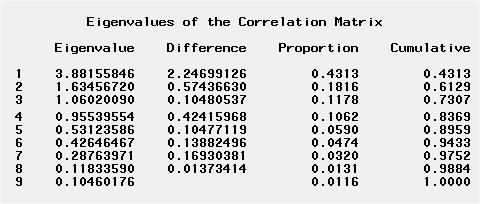
\includegraphics[scale=0.9]{3AEigen.jpg}\\
		\caption{Eigenvalue Table}\label{Eigenvalue Table}
	\end{center}
	
\end{figure}


\subsubsection{Advantages and Disadvantages}

The proportion of variance criterion has a number of positive features.  For example, in most
cases, you would not want to retain a group of components that, combined, account for only a
minority of the variance in the data set (say, $30\%$).  Nonetheless, many critical values discussed
earlier are obviously arbitrary.  Because of these and related problems, this approach has sometimes been
criticized for its subjectivity (Kim and Mueller, 1978).

\subsection{The Interpretability Criteria}

Perhaps the most important criterion for solving the \textbf{\emph{number of-components}} problem is the interpretability criterion:  interpreting the substantive meaning of the retained components and verifying that this interpretation makes sense in terms of what is known about the constructs under investigation.


The following list provides four rules to follow in doing this. \\ (A later section shows how to
actually interpret the results of a principal component analysis; the following rules will be more
meaningful after you have completed that section).

\begin{enumerate}
	\item Are there at least three variables (items) with significant loadings on each retained
	component?  A solution is less satisfactory if a given component is measured by less than
	three variables.
	
	\item  Do the variables that load on a given component share the same conceptual meaning?
	For example, if three questions on a survey all load on component 1, do all three of these
	questions seem to be measuring the same construct?
	
	\item  Do the variables that load on different components seem to be measuring different
	constructs?  For example, if three questions load on component 1, and three other
	questions load on component 2, do the first three questions seem to be measuring a
	construct that is conceptually different from the construct measured by the last three
	questions?
	
	\item  Does the rotated factor pattern demonstrate “simple structure?”  Simple structure
	means that the pattern possesses two characteristic:
	
	\begin{itemize}
		\item[(a)] Most of the variables have
		relatively high factor loadings on only one component, and near zero loadings on the other
		components, and \item[(b)] most components have relatively high factor loadings for some
		variables, and near-zero loadings for the remaining variables.
	\end{itemize}
\end{enumerate}
\newpage
%----------------------------------------------------------------------------------%
\section{Review of Important Definitions}
\begin{itemize}
	\item An observed variable can be measured directly, is sometimes called a measured variable or an indicator or a
	manifest variable.
	\item A principal component is a linear combination of weighted observed variables. Principal components are
	uncorrelated and orthogonal.
	\item A latent construct can be measured indirectly by determining its influence to responses on measured variables. A latent construct could is also referred to as a factor, underlying construct, or unobserved variable.
	\item Factor scores are estimates of underlying latent constructs.
	\item Unique factors refer to unreliability due to measurement error and variation in the data.
	\item Principal component analysis minimizes the sum of the squared perpendicular distances to the axis of the
	principal component while least squares regression minimizes the sum of the squared distances perpendicular to the
	x axis (not perpendicular to the fitted line).
	\item Principal component scores are actual scores.
	\item Eigenvectors are the weights in a linear transformation when computing principal component scores.
	Eigenvalues indicate the amount of variance explained by each principal component or each factor.
	\item Orthogonal means at a 90 degree angle, perpendicular.
	Obilque means other than a 90 degree angle.
	\item An observed variable \textbf{\emph{loads}} on a factors if it is highly correlated with the factor, has an eigenvector of greater magnitude on that factor.
	\item Communality is the variance in observed variables accounted for by a common factors. Communality is more
	relevant to EFA than PCA.
\end{itemize}
\newpage

\begin{itemize}
	\item \texttt{princomp}
	\item \texttt{prcomp}
	\item
\end{itemize}
%================================================%
\newpage

\[ \mbox{ } \]

%================================================%
\newpage

\begin{framed}
	\begin{verbatim}
	Proportion of Variance 0.6200604 0.2474413 0.0891408 0.04335752
	Cumulative Proportion  0.6200604 0.8675017 0.9566425 1.00000000
	> loadings(pc.cr)  
	
	# note that blank entries are small but not zero
	
	Loadings:
	Comp.1 Comp.2 Comp.3 Comp.4
	Murder   -0.536  0.418 -0.341  0.649
	Assault  -0.583  0.188 -0.268 -0.743
	UrbanPop -0.278 -0.873 -0.378  0.134
	Rape     -0.543 -0.167  0.818       
	
	Comp.1 Comp.2 Comp.3 Comp.4
	SS loadings      1.00   1.00   1.00   1.00
	Proportion Var   0.25   0.25   0.25   0.25
	Cumulative Var   0.25   0.50   0.75   1.00
	\end{verbatim}
\end{framed}
%=========================================%
\newpage
\begin{framed}
	\begin{verbatim}
	## The signs of the columns are arbitrary
	> plot(pc.cr) # shows a screeplot.
	> biplot(pc.cr)
	> 
	> ## Formula interface
	> princomp(~ ., data = USArrests, cor = TRUE)
	Call:
	princomp(formula = ~., data = USArrests, cor = TRUE)
	
	Standard deviations:
	Comp.1    Comp.2    Comp.3    Comp.4 
	1.5748783 0.9948694 0.5971291 0.4164494 
	
	4  variables and  50 observations.
	
	
	\end{verbatim}
\end{framed}
%================================================%
\newpage
\begin{framed}
	\begin{verbatim}
	> ## NA-handling
	> USArrests[1, 2] <- NA
	> pc.cr <- princomp(~ Murder + Assault + UrbanPop,
	+                   data = USArrests, na.action = na.exclude, 
	cor = TRUE)
	> 
	\end{verbatim}
\end{framed}
%================================================%
\subsection*{\texttt{prcomp}}
Performs a principal components analysis on the given data matrix and returns the results as an object of class \texttt{prcomp}.

\newpage
\begin{framed}
	\begin{verbatim}
	> prcomp(~ Murder + Assault + Rape, 
	data = USArrests, scale = TRUE)
	Standard deviations:
	[1] 1.5380939 0.6691898 0.4318010
	
	Rotation:
	PC1        PC2        PC3
	Murder  -0.5822314  0.5349197 -0.6122643
	Assault -0.6063988  0.2159081  0.7652870
	Rape    -0.5415599 -0.8168504 -0.1986662
	\end{verbatim}
\end{framed}
%=========================================================================== %
\newpage
\section{Singular Value Decomposition (SVD)}
\textit{Source: : http://iridl.ldeo.columbia.edu/dochelp/StatTutorial/SVD/ \\}
Singular value decomposition (SVD) is quite possibly the most widely-used multivariate statistical technique used in the atmospheric sciences. The technique was first introduced to meteorology in a 1956 paper by Edward Lorenz, in which he referred to the process as empirical orthogonal function (EOF) analysis. Today, it is also commonly known as principal-component analysis (PCA). All three names are still used, and refer to the same set of procedures within the Data Library. 


The purpose of singular value decomposition is to reduce a dataset containing a large number of values to a dataset containing significantly fewer values, but which still contains a large fraction of the variability present in the original data. Often in the atmospheric and geophysical sciences, data will exhibit large spatial correlations. SVD analysis results in a more compact representation of these correlations, especially with multivariate datasets and can provide insight into spatial and temporal variations exhibited in the fields of data being analyzed. 


There are a few caveats one should be aware of before computing the SVD of a set of data. First, the data must consist of anomalies. Secondly, the data should be de-trended. When trends in the data exist over time, the first structure often captures them. If the purpose of the analysis is to find spatial correlations independent of trends, the data should be de-trended before applying SVD analysis. 

\newpage

\subsection*{Question 5}
Load the hand-written digits data using the following commands:

\begin{framed}
	\begin{verbatim}
	library(ElemStatLearn)
	data(zip.train)
	\end{verbatim}
\end{framed}

Each row of the `\texttt{zip.train}` data set corresponds to a hand written digit. The
first column of the zip.train data is the actual digit. The next 256 columns
are the intensity values for an image of the digit. To visualize the digit we
can use the `\texttt{zip2image()}` function to convert a row into a 16 x 16 matrix:

\begin{framed}
	\begin{verbatim}
	# Create an image matrix for the 3rd row, which is a 4
	im = zip2image(zip.train,3)
	image(im)
	\end{verbatim}
\end{framed}


Using the `zip2image` file, create an image matrix for the 8th and 18th rows.
\begin{figure}
	\centering
	\includegraphics[width=0.7\linewidth]{./DAquiz3Graph5b}
	\caption{}
	\label{fig:DAquiz3Graph5}
\end{figure}
For each image matrix calculate the `\textit{\textbf{svd}}` of the matrix (with no scaling). 

\begin{itemize}
	\item[(i)] What is the percent variance explained by the \textbf{first} singular vector for the image
	from the 8th row? 
	\item[(ii)] What is the percent variance explained for the image from the
	18th row? (by the \textbf{first} singular vector)
	\item[(iii)] Why is the percent variance lower for the image from the 18th row?
\end{itemize}
\newpage
\begin{framed}
	\begin{verbatim}
	
	im8 <- zip2image(zip.train, 8)
	im18 <- zip2image(zip.train, 18)
	
	svd8 <- svd(im8)
	svd18 <- svd(im18)
	
	par(mfrow=c(2,2))
	plot(svd8$d^2/sum(svd8$d^2),
	xlab="Column",ylab="Percent of variance explained for Row 8",
	pch=19)
	
	plot(svd18$d^2/sum(svd18$d^2),
	xlab="Column",ylab="Percent of variance explained for Row 18",
	pch=19)
	
	image(im8)
	
	image(im18)
	
	\end{verbatim}
\end{framed}
\newpage
From the image - the second image is more complicated, so there are multiple patterns each explaining a large percentage of variance.
\begin{figure}[h!]
	\centering
	\includegraphics[width=1.0\linewidth]{./DAquiz3Graph5b}
	\caption{}
	\label{fig:DAquiz3Graph5}
\end{figure}

\end{document}
~~The first singular vector explains 98\% of the variance for row 8 and 48\% for row 18. 
The reason the first singular vector explains less variance for the 18th row is because the 8th row has higher average values.~~
**The first singular vector explains 98\% of the variance for row 8 and 48\% for row 18. 
The reason the first singular vector explains less variance for the 18th row is that the image is more complicated, so there are multiple patterns each explaining a large percentage of variance.**

\end{document}
